\begin{samplecase}
{\bf Pre-equilibrium angular dist. and multiple pre-equilibrium emission}\newline

At high incident energies, multiple pre-equilibrium reactions play a
significant role. In this sample case, we show the results for this
mechanism in the output file. Also, as an alternative to the previous
sample case, we present another way of producing
double-differential cross sections, namely as a function of angle at a fixed
outgoing energy. With the following input file, the reaction of 120 MeV protons
incident on ${}^{90}$Zr is simulated:

\VerbatimInput{\samples p-Zr090-preeq/org/talys.inp}

The results are presented in Figs.~\ref{spec120} and \ref{pddx120}.
For this sample case, since {\bf outpopulation y},
after each print of the population for each residual nucleus (as already
described in the first sample case), a block with multiple pre-equilibrium
decay information is printed.
This output block begins with
{\small \begin{verbatim}
 Multiple preequilibrium emission from Z= 41 N= 49 ( 90Nb):

                                                             Feeding terms from

 bin    Ex  Mpe ratio  neutron   proton   1 1 0 0   0 0 1 1   1 0 0 1   0 1 1 0
                      emission  emission

  11   2.208 0.00000 0.000E+00 0.000E+00 0.000E+00 0.000E+00 5.287E-01 0.000E+00
  12   4.980 0.00000 0.000E+00 0.000E+00 0.000E+00 0.000E+00 1.249E+00 0.000E+00
  13   7.752 0.00000 0.000E+00 0.000E+00 0.000E+00 0.000E+00 1.961E+00 0.000E+00
  14  10.524 0.00001 0.000E+00 4.343E-05 0.000E+00 0.000E+00 2.645E+00 0.000E+00
  15  13.296 0.00555 3.214E-04 1.999E-02 0.000E+00 0.000E+00 3.300E+00 0.000E+00
  16  16.067 0.04999 5.901E-03 2.049E-01 0.000E+00 0.000E+00 3.928E+00 0.000E+00
  17  18.839 0.10870 2.305E-02 5.024E-01 0.000E+00 0.000E+00 4.527E+00 0.000E+00
  18  21.611 0.17335 5.014E-02 8.952E-01 0.000E+00 0.000E+00 5.098E+00 0.000E+00
.....................................
\end{verbatim} } \renewcommand{\baselinestretch}{1.07}\small\normalsize
\noindent
For each continuum bin, with excitation energy $E_{x}$, we print the fraction
of the population that is emitted as multiple pre-equilibrium. Also the total
neutron
and proton emission per residual nucleus is printed, as well as the feeding
terms from previous particle-hole configurations.
With this input file, files {\em nspec120.000.tot} and {\em pspec120.000.tot}
are created through the {\em filespectrum n p} keyword. The results are
displayed in Fig.~\ref{spec120}.
Also, the combination of {\bf ddxmode 1} and the various {\bf fileddxe} keywords
generate the {\em pddx100.0.mev}, etc. files that are compared with experimental
data in Fig.~\ref{pddx120}.

\end{samplecase}
\begin{figure}
\centering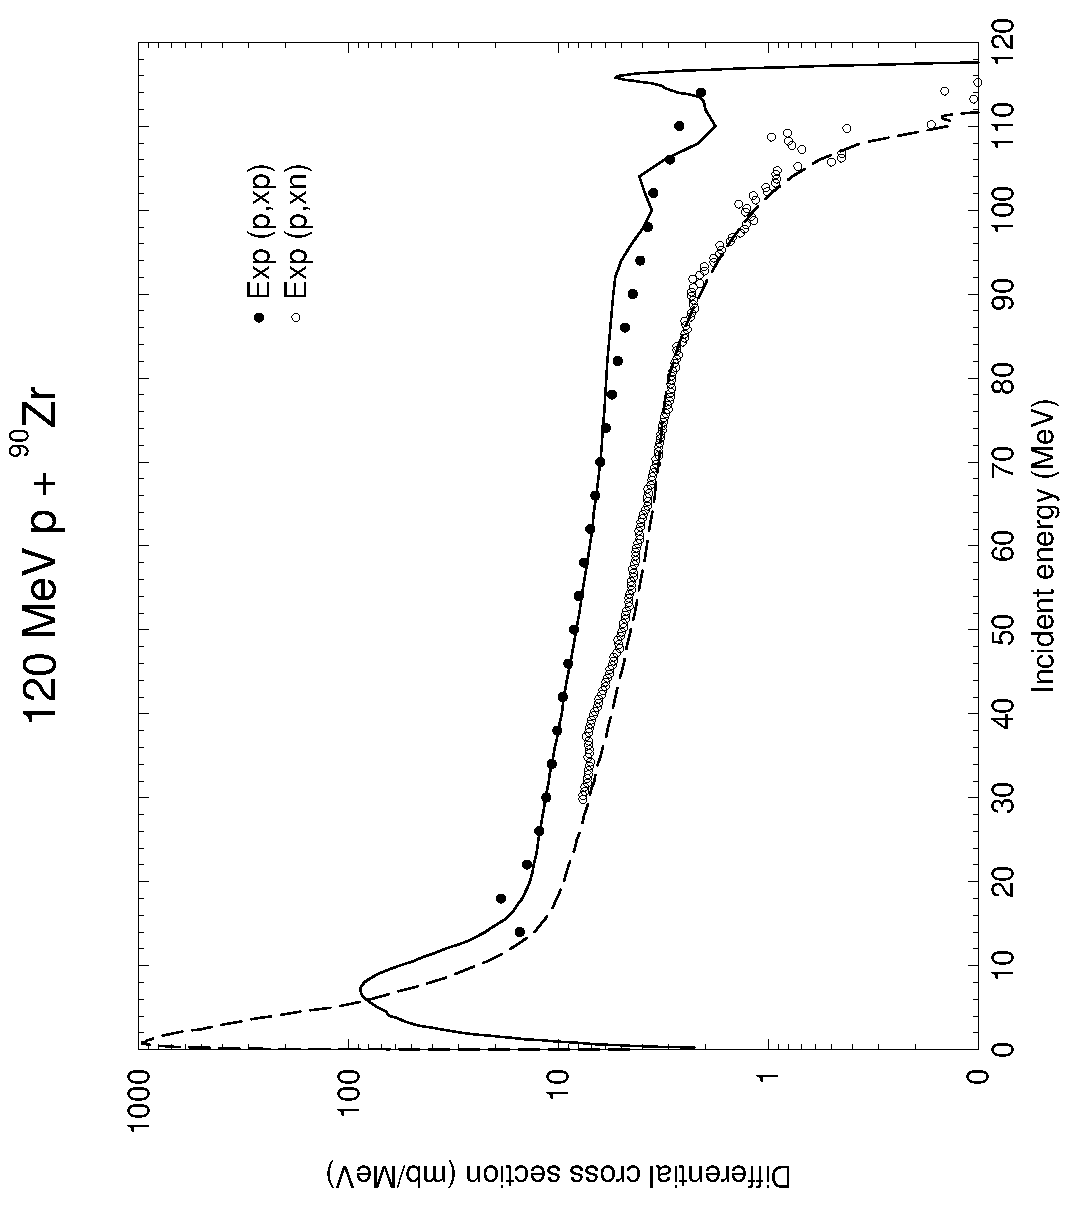
\includegraphics[scale=0.5,angle=270]{spec120}
\caption{Angle-integrated (p,xn) and (p,xp) spectra for 120 MeV protons
on ${}^{90}$Zr. Experimental data are taken from \protect\cite{Cowley1991,Scobel1990}}
\label{spec120}
\end{figure}
\begin{figure}
\centering\includegraphics[scale=0.5,angle=270]{pddx120}
\caption{Double-differential (p,xp) spectra for 120 MeV protons
on ${}^{90}$Zr. Experimental data are taken from \protect\cite{Cowley1991} }
\label{pddx120}
\end{figure}
